\documentclass[12pt]{article}

\usepackage[utf8]{inputenc}
\usepackage[T1]{fontenc}
\usepackage{amsmath}
\usepackage{amssymb}
\usepackage{amsthm}
\usepackage{graphicx}
\usepackage{hyperref}
\usepackage{geometry}

\geometry{
    a4paper,
    margin=2.5cm
}

\title{Analysis of Neural Tangent Kernel for Matrix Multiplication Neural Networks}
\author{Your Name}
\date{\today}

\begin{document}

\maketitle

\begin{abstract}
This document presents an analysis of the Neural Tangent Kernel (NTK) for Matrix Multiplication Neural Networks (MMNNs). We focus on two-layer architectures with ReLU activation functions and examine the NTK behavior under various conditions, including different ranks, sample sizes, and values of the parameter $\beta$. Our results indicate that the NTK standard deviation decreases rapidly with rank, making the mean NTK increasingly deterministic. This property enables reliable analysis of the kernel behavior. We also analyze the NTK distribution, its spectrum, and its dependence on hyperparameters, revealing characteristic behaviors of MMNNs.
\end{abstract}

\section{Introduction}
The study of Neural Tangent Kernels (NTK) has provided profound insights into the behavior of deep neural networks, particularly in the infinite-width limit where the training dynamics can be described by a kernel. This analysis is grounded in the fact that, in this limit, the pre-activation outputs of the first layer follow a Gaussian Process. While the NTK for standard architectures like Multi-Layer Perceptrons (MLPs) is well-understood, its properties for more complex models like Matrix Multiplication Neural Networks (MMNNs) remain less explored.

In this work, I conduct a detailed empirical investigation of the NTK for two-layer MMNNs with ReLU activations. My goal is to characterize the NTK's dependence on two critical hyperparameters: the internal rank of the matrix multiplication and a bias-like parameter, $\beta$. I aim to understand how these parameters affect not only the average behavior of the kernel but also its statistical fluctuations.

\section{Experimental Methodology}
My experimental setup was designed to systematically explore the parameter space of the MMNNs and their corresponding NTK.

\subsection{Model Architecture and Data}
\begin{itemize}
    \item \textbf{Model:} I use a two-layer MMNN with a ReLU activation function, $\sigma(x) = \max(0, x)$, where the first layer has a width of 1000. The network produces a scalar, one-dimensional output.
    \item \textbf{Data:} My input vectors are two-dimensional and sampled uniformly from the unit sphere. I chose this low-dimensional setup because the NTK is a zonal kernel, meaning it only depends on the scalar product $\rho = x^T x'$ between inputs. This allows for extensive and expressive experiments without suffering from the curse of dimensionality.
\end{itemize}

\subsection{Hyperparameter Configuration}
\begin{itemize}
    \item \textbf{Rang interne ($r$) :} Le rang de la décomposition matricielle est un paramètre central, varié sur une échelle logarithmique (de 2 à 100). La matrice de poids de la seconde couche est normalisée par $1/\sqrt{r}$.
    \item \textbf{Paramètre $\beta$ :} Contrairement aux analyses standards de MLPs où $\beta$ est souvent nul, nous explorons des valeurs non nulles pour étudier son influence non triviale sur le noyau.
\end{itemize}
Chaque configuration expérimentale est un n-uplet (dimension, nombre de points $n$, $\beta$, rang $r$).

\subsection{NTK Computation and Statistical Estimation}
I estimate the NTK using a Monte Carlo method. This approach is a practical necessity. The exact analytical computation would require an integration over a high-dimensional Gaussian measure associated with the weights of the second layer (where the dimension is the rank $r$), which is computationally intractable.
\begin{itemize}
    \item I use 300 random points for the Monte Carlo estimation. Care was taken to resample the weight matrices for each draw to ensure statistical independence.
    \item For each configuration, I compute 50 distinct NTK matrices over a fixed dataset. This allows me to perform a statistical analysis of the kernel itself.
    \item Given the uniform sampling, I also employed bootstrapping techniques to generate a richer dataset for more robust density visualizations and statistical estimations of quantities like the mean and standard deviation.
\end{itemize}

\section{Results and Observations}

\subsection{Impact of Internal Rank on NTK Statistics}
My most significant observation is that the standard deviation of the NTK entries (both diagonal and off-diagonal) decays as a power law with the internal rank $r$ (Figure \ref{fig:rank_scaling}). This is a powerful finding. It means that as the rank grows, the NTK's random component vanishes, and the kernel becomes increasingly deterministic. Consequently, I can confidently use the mean NTK, $\mathbb{E}[\Theta]$, as a reliable representation of its behavior for my analysis. This is fantastic because it allows me to condition integrals well, even within deep Gaussian processes.

I also noted that for low ranks, the NTK spectrum is enhanced with many positive eigenvalues that are of the same order of magnitude as the leading one (Figure \ref{fig:min_ntk}).

\begin{figure}[h!]
    \centering
    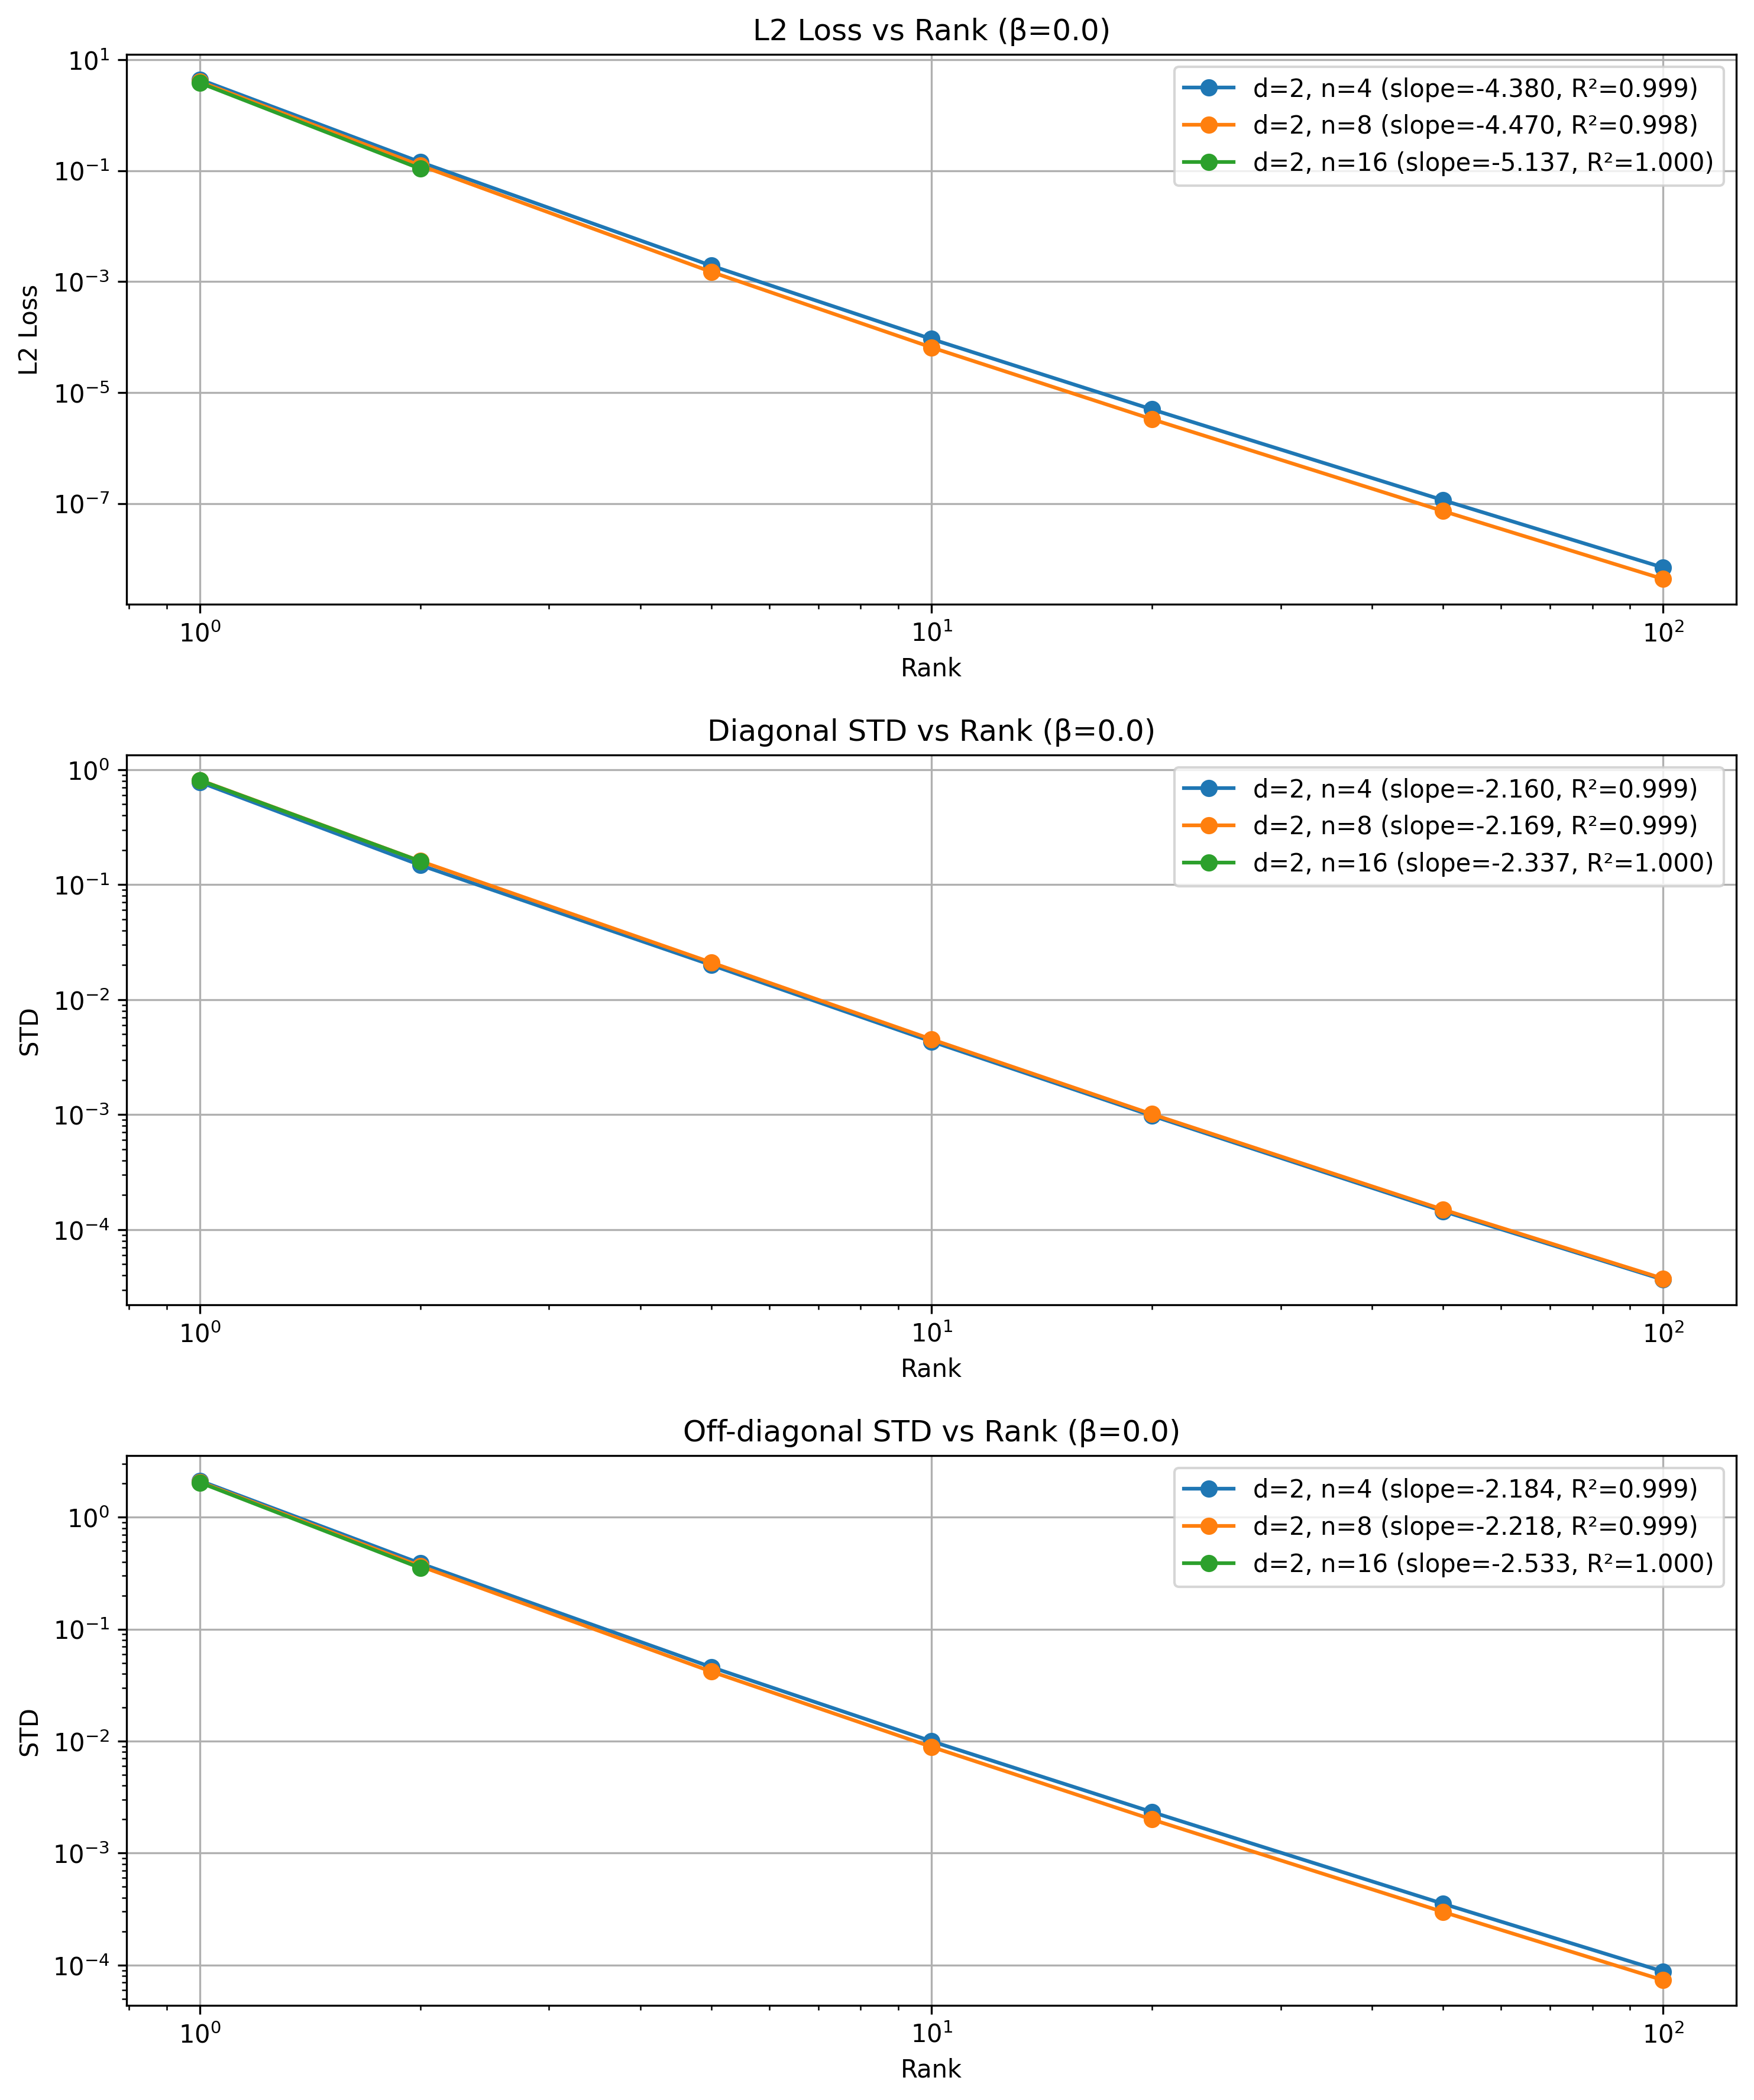
\includegraphics[width=0.7\textwidth]{figures/rank_scaling_beta0.png}
    \caption{Decay of the NTK's standard deviation as a function of rank for $\beta=0$.}
    \label{fig:rank_scaling}
\end{figure}

\begin{figure}[h!]
    \centering
    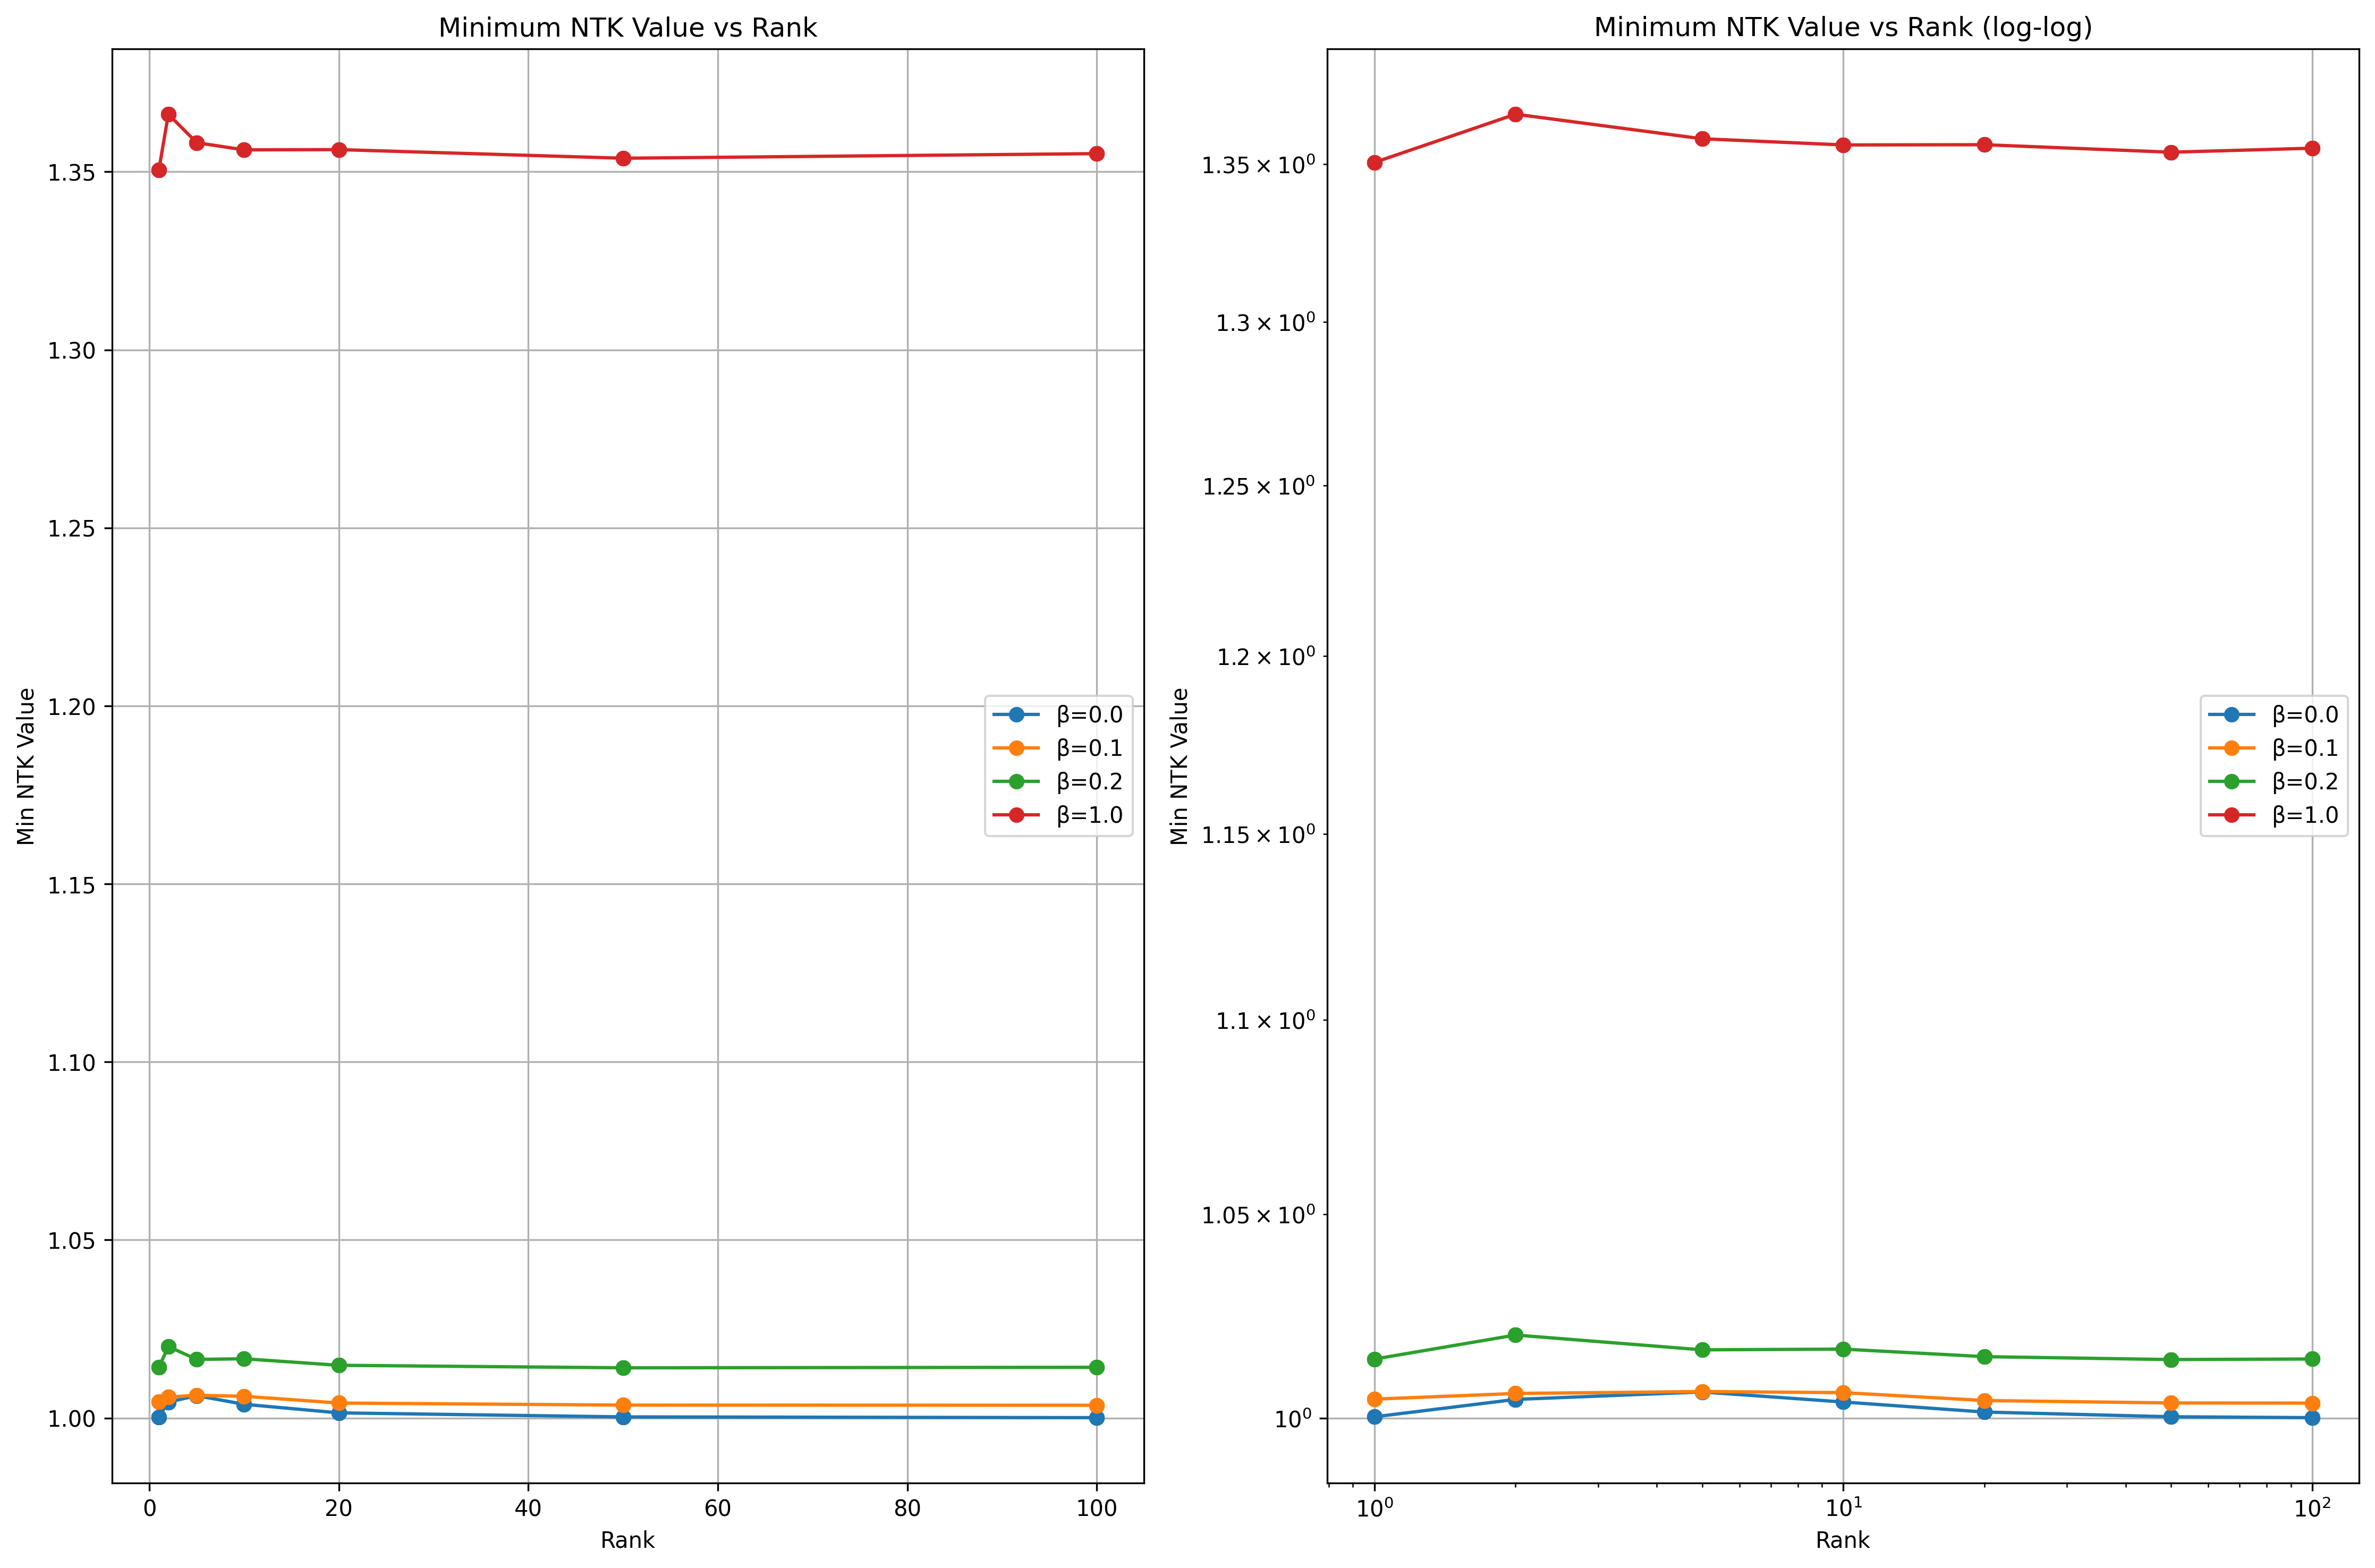
\includegraphics[width=0.7\textwidth]{figures/min_ntk_vs_rank.png}
    \caption{Behavior of the smallest NTK eigenvalue as a function of rank.}
    \label{fig:min_ntk}
\end{figure}


\subsection{Dependence on the $\beta$ Parameter}
The $\beta$ parameter has a very clear impact. For $\beta = 0$, I observed that the mean NTK value converges towards 0 with a particular slope as rank increases. For $\beta > 0$, it converges to a non-zero constant. My plots indicate that the dependence of this limit on $\beta$ appears to be either linear or quadratic (Figure \ref{fig:conv_beta}). I am confident this limit can be computed theoretically, although it would require integrating special functions (like `erf` and Gaussian CDFs), which I also plan to verify numerically in Python.

\begin{figure}[h!]
    \centering
    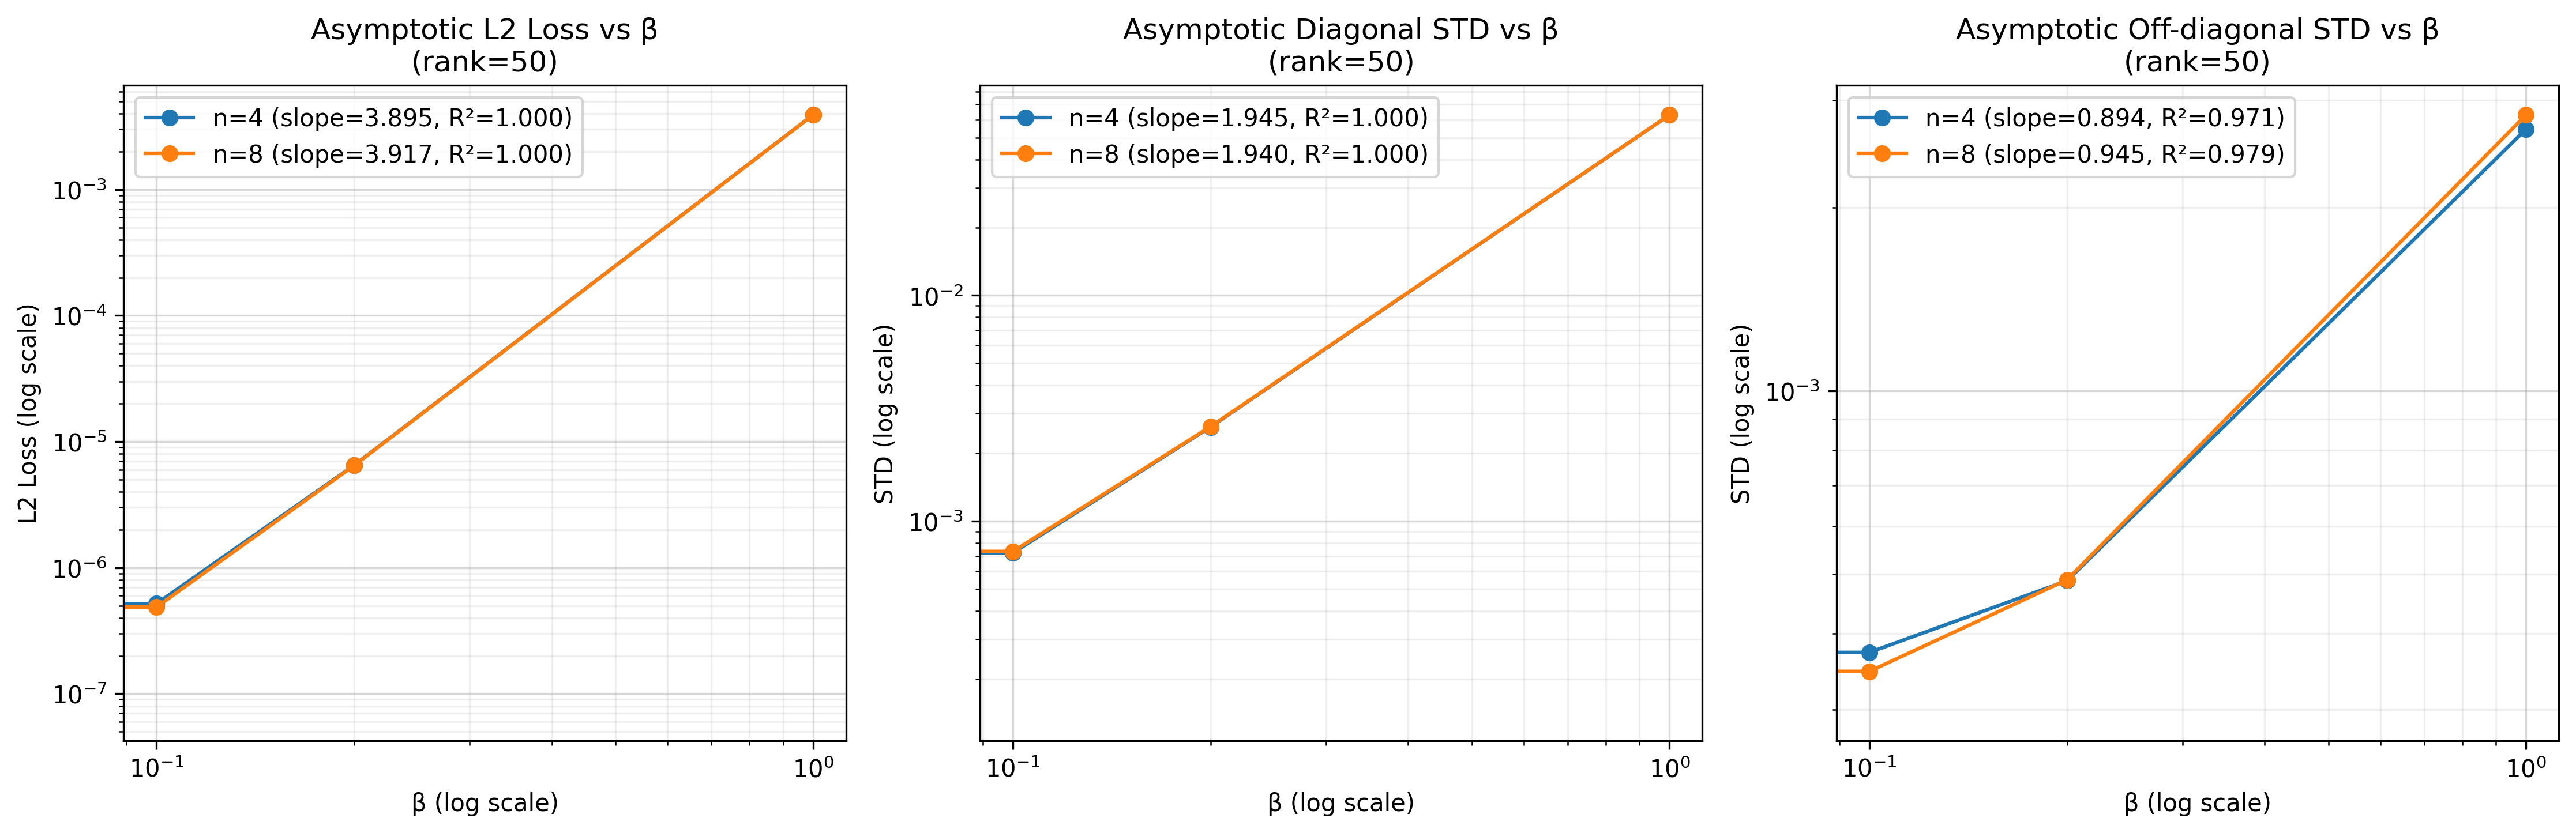
\includegraphics[width=0.49\textwidth]{figures/convergence_vs_beta_rank50.png}
    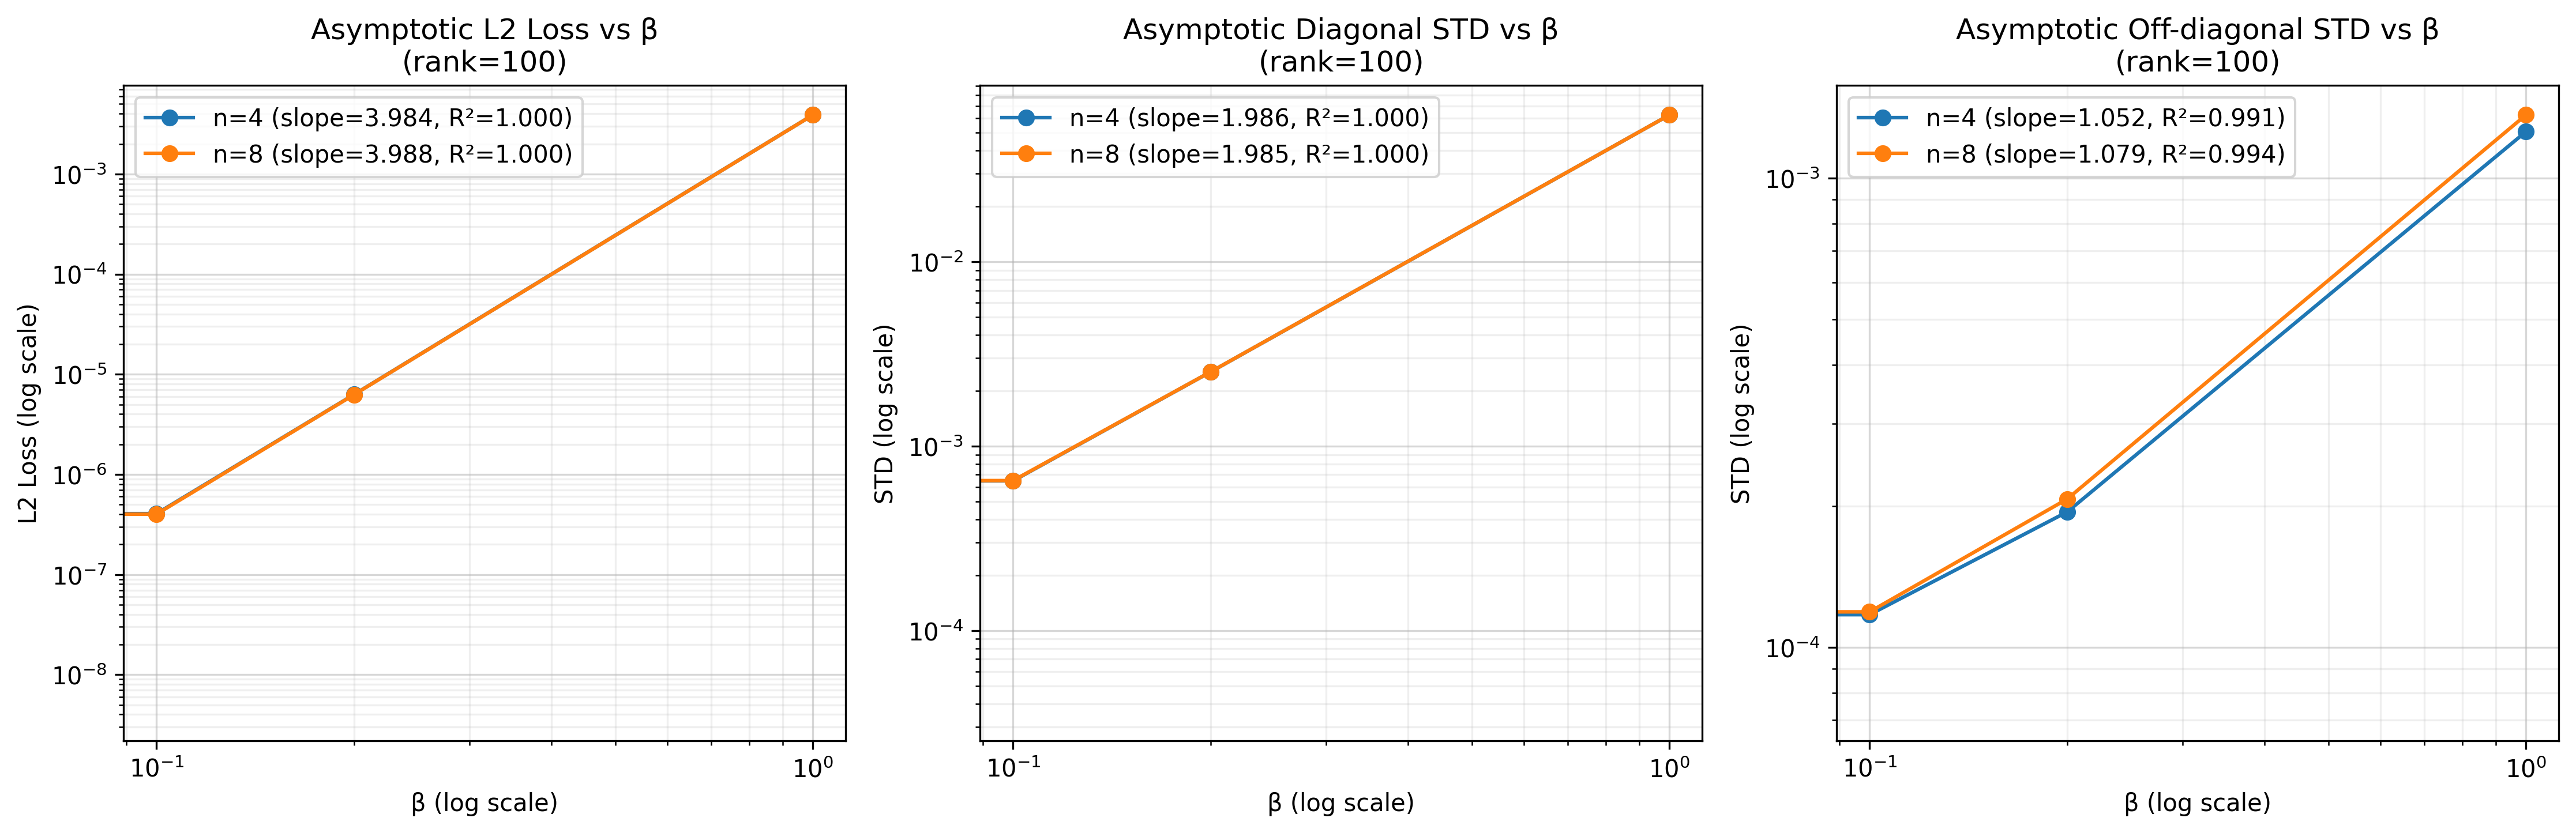
\includegraphics[width=0.49\textwidth]{figures/convergence_vs_beta_rank100.png}
    \caption{Convergence of the mean NTK as a function of $\beta$ for rank 50 (left) and 100 (right).}
    \label{fig:conv_beta}
\end{figure}


\subsection{Distributional Analysis of the NTK}
I analyzed the distribution of NTK values, conditioned on the dot product $\rho$ (Figure \ref{fig:dist_rho}). Using various kernel density estimators (Epanechnikov, Gaussian, etc.), I made several key observations.
\begin{itemize}
    \item The distributions exhibit heavy, power-law-like tails, especially at low ranks (Figure \ref{fig:loglog_kde}). I am currently in the process of formally verifying this using Hill estimators.
    \item The distribution of the on-diagonal elements is particularly interesting; while it tends towards a Gaussian with rank, it also exhibits a pyramid-like shape, which suggests a potential connection to Random Matrix Theory.
    \item The off-diagonal elements show a tailed distribution with a mode concentrated near 1 for lower ranks, which then converges to a Gaussian as the rank increases.
    \item Despite the heavy tails at low ranks, the overall distribution clearly converges towards a Gaussian as the rank grows, as shown in Figure \ref{fig:dist_rank}, which is consistent with the Central Limit Theorem.
\end{itemize}

\begin{figure}[h!]
    \centering
    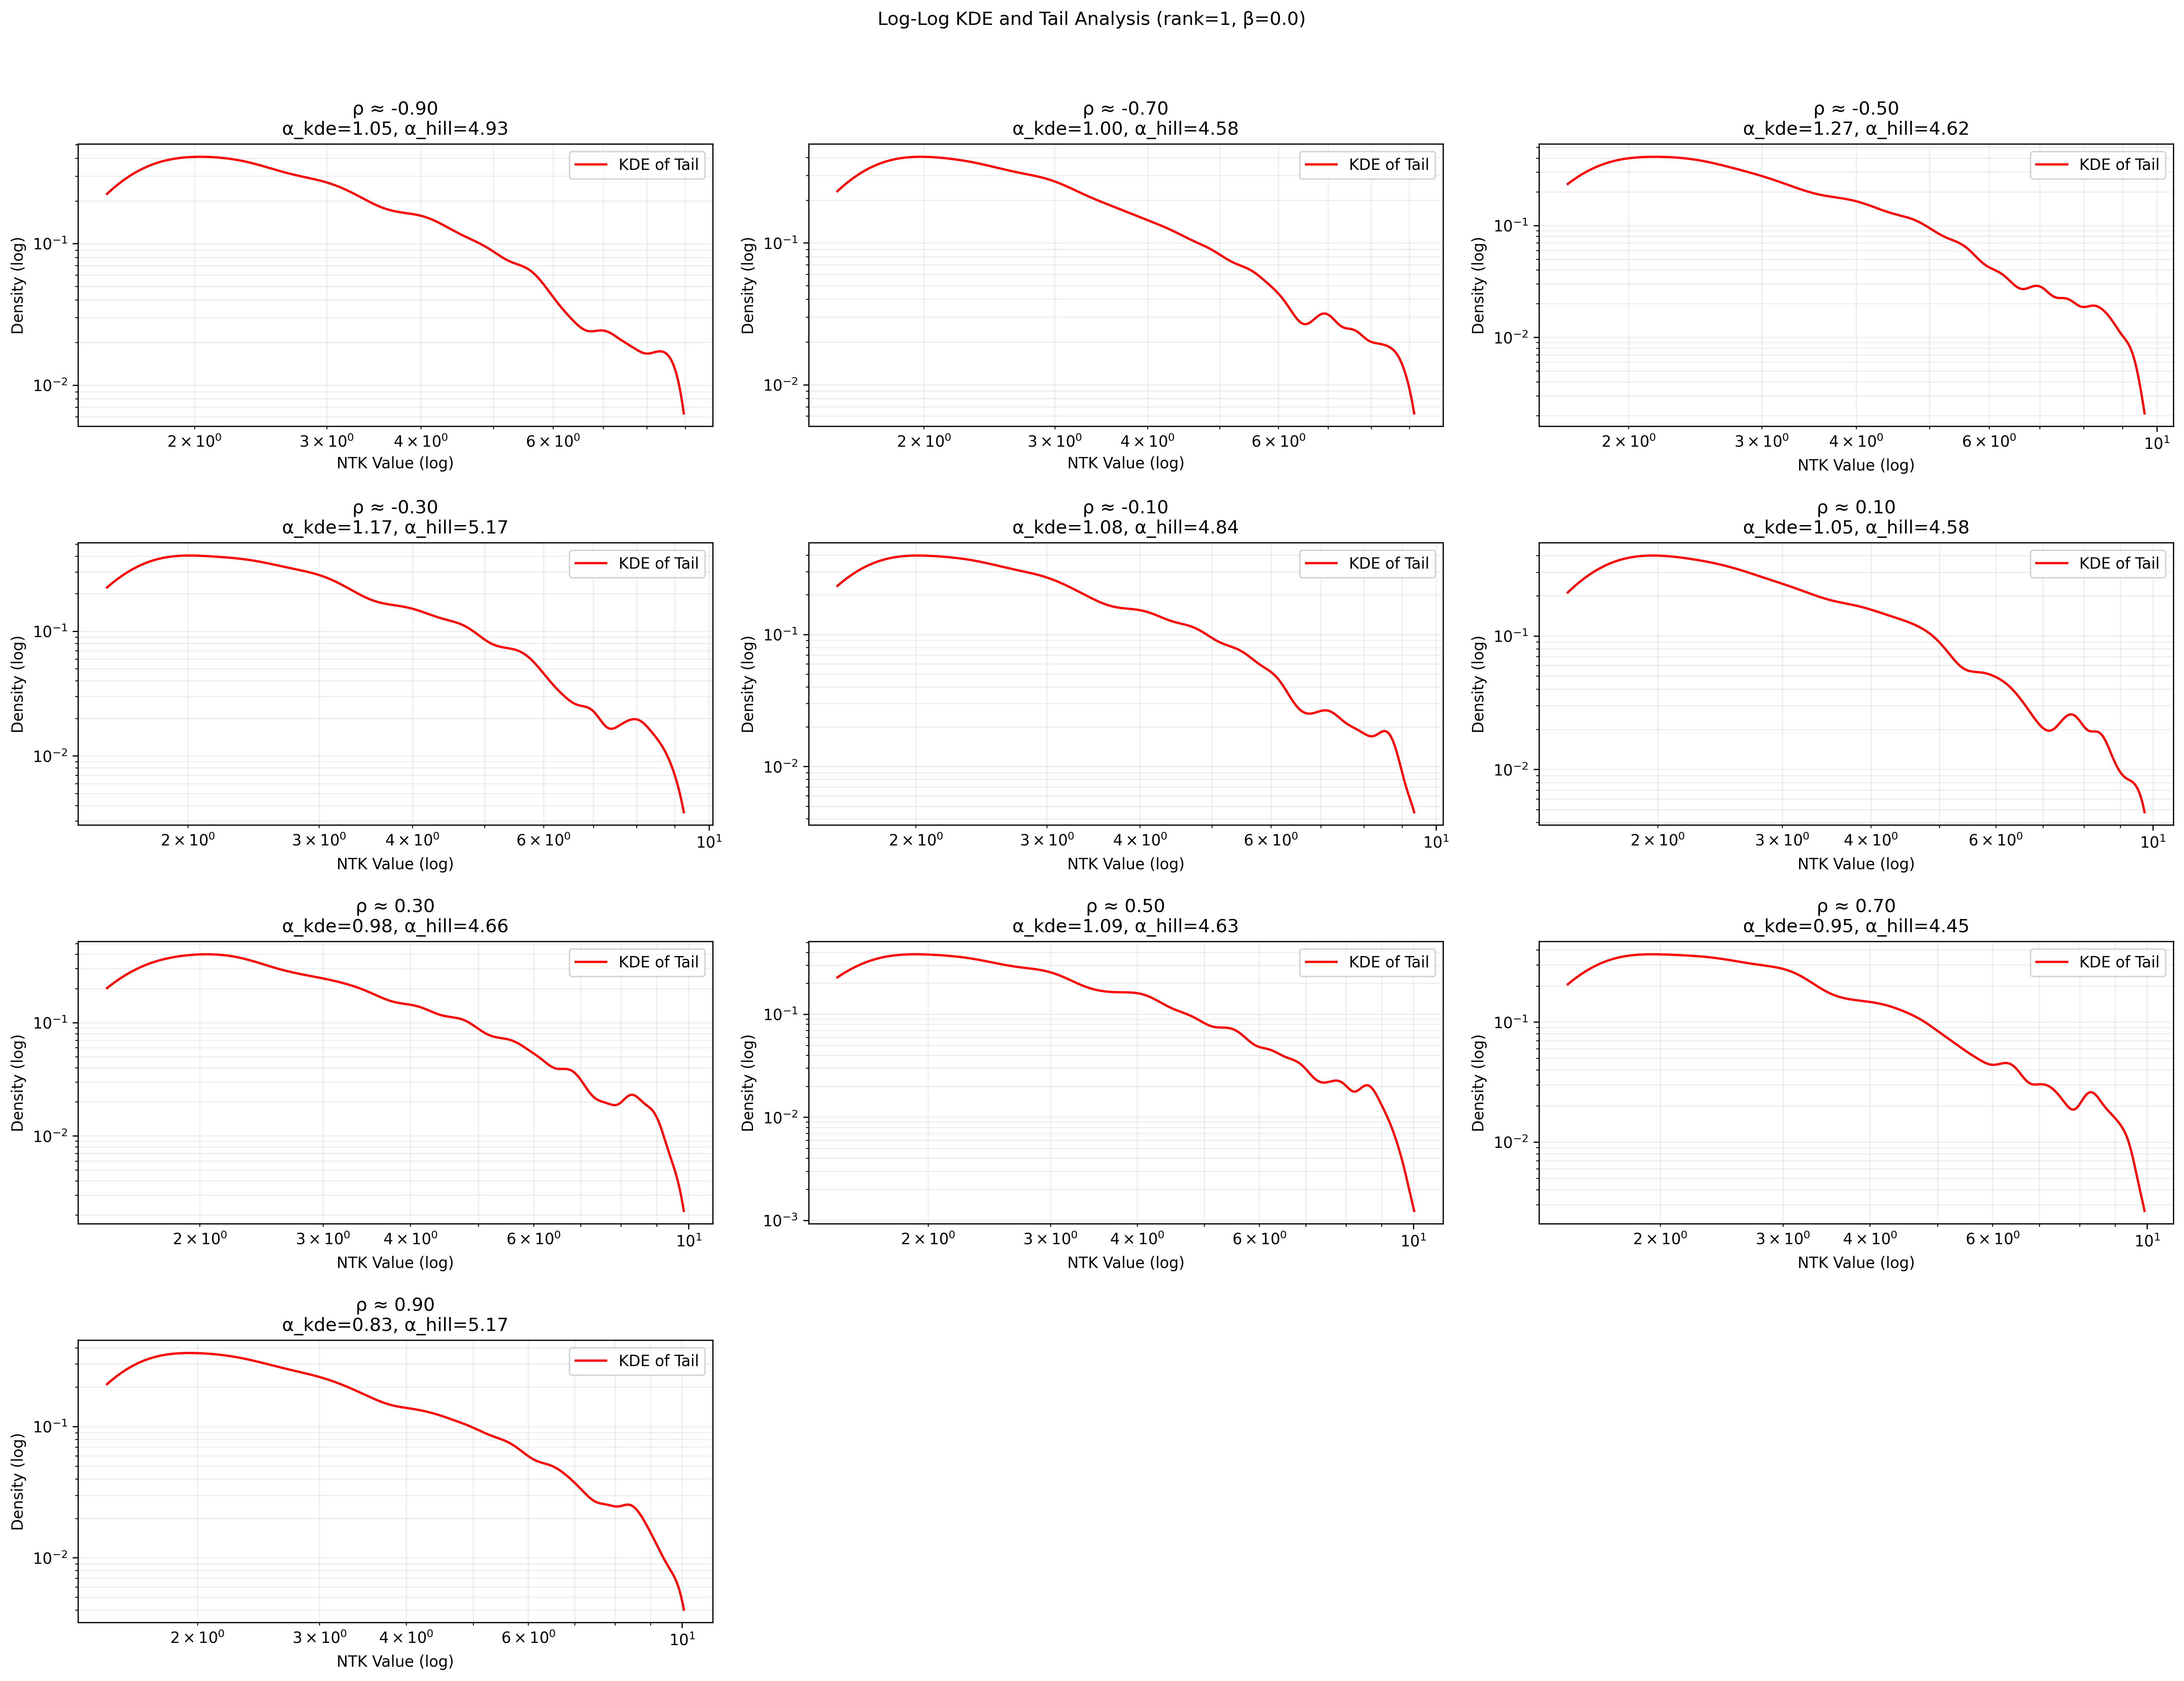
\includegraphics[width=0.7\textwidth]{figures/ntk_loglog_kde_rank1_beta0.0_gaussian.png}
    \caption{Log-log scale plot of the NTK's probability density (KDE), suggesting a power-law tail for low rank.}
    \label{fig:loglog_kde}
\end{figure}

\begin{figure}[h!]
    \centering
    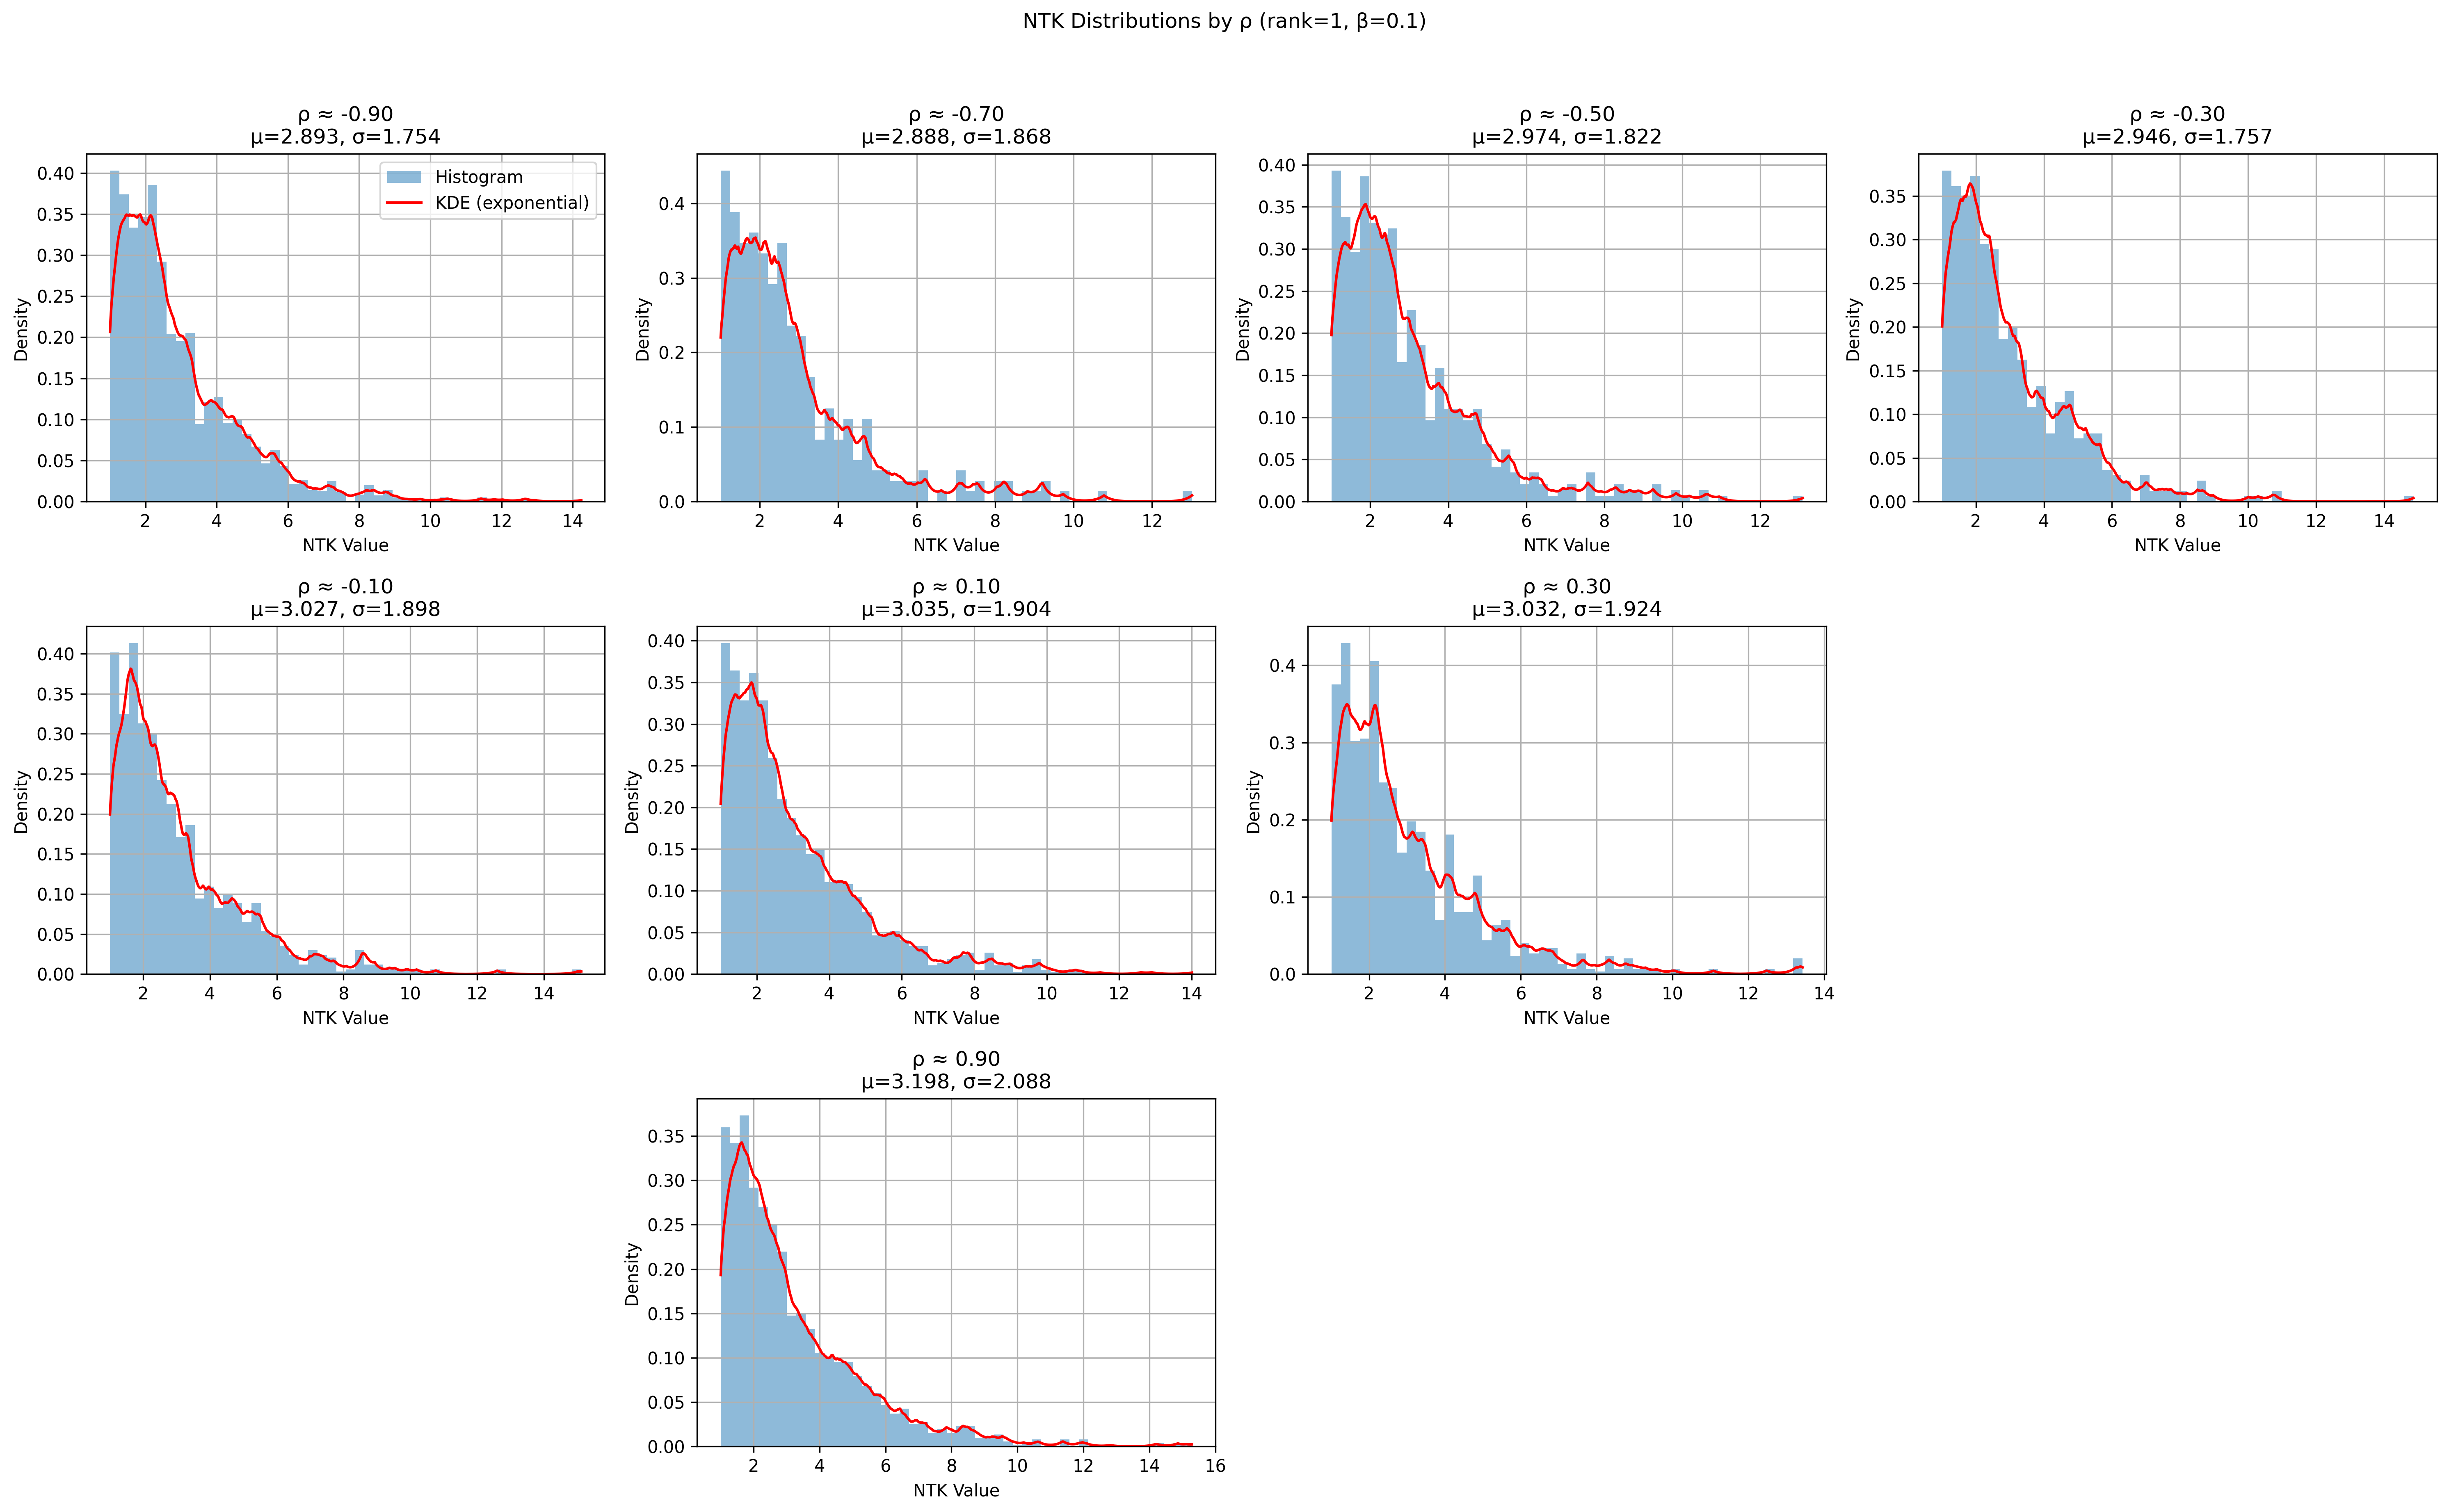
\includegraphics[width=0.7\textwidth]{figures/ntk_distributions_by_rho_rank1_beta0.1_exponential_bw0.2.png}
    \caption{Distribution of NTK values as a function of $\rho$.}
    \label{fig:dist_rho}
\end{figure}

\begin{figure}[h!]
    \centering
    
\includegraphics[width=0.49\textwidth]{figures/ntk_distributions_rank2_beta1.0_gaussian.png}
    
\includegraphics[width=0.49\textwidth]{figures/ntk_distributions_rank5_beta1.0_gaussian.png}
    \caption{Convergence of the NTK distribution towards a Gaussian as rank increases (from 2 to 5).}
    \label{fig:dist_rank}
\end{figure}


\subsection{Mean NTK and Structural Properties}
When I plotted the mean NTK as a function of the input dot product $\rho$, I noticed a very low degree of convexity. Specifically, for high ranks like $r=100$, the relationship is nearly linear with a high R-squared value.

I also compared the spectral properties of these architectures. I found that the spectrum of the empirical NTK for a 1-layer MMNN shows a remarkable similarity to the theoretical NTK spectrum of a 2-layer MLP, but scaled by a factor of $1/2$ (Figure \ref{fig:comparison_mlp}). The "gain" from adding a second layer to the MMNN appears to correspond to the contributions of two specific terms in the NTK's recurrence formula.

Furthermore, I remarked that the NTK matrix exhibits a compound structure. To quantify this, I computed its L2 loss over this specific subspace, confirming a structured deviation from a simpler matrix form.

\begin{figure}[h!]
    \centering
    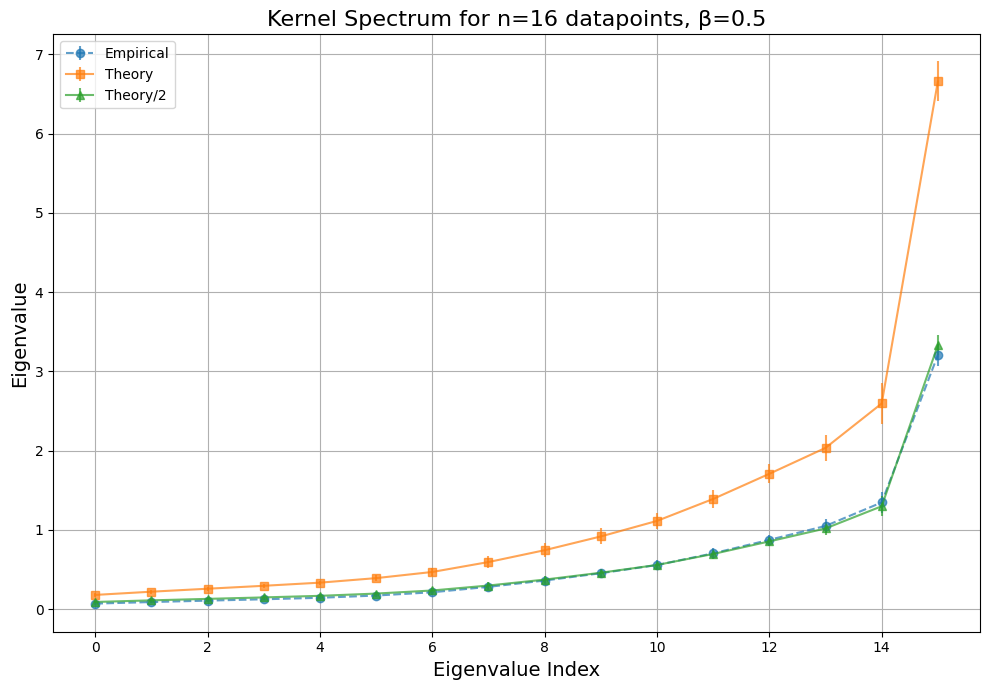
\includegraphics[width=0.7\textwidth]{figures/kernelspectrum_mlp_mmnn.png}
    \caption{Comparison of kernel spectra. The empirical spectrum for a 1-layer MMNN is compared against the theoretical spectrum for a 2-layer MLP.}
    \label{fig:comparison_mlp}
\end{figure}


\section{Conclusion}
In conclusion, my empirical analysis has uncovered several distinct properties of the NTK for MMNNs. The most critical result is the rapid decay of the NTK's variance with increasing internal rank. This concentration phenomenon implies that for sufficiently high ranks, the NTK behaves like a deterministic kernel that can be fully characterized by its mean. This is a powerful conclusion, as it greatly simplifies the theoretical analysis of these models. Furthermore, I have characterized the significant influence of the $\beta$ parameter and identified unique signatures in the kernel's functional form that distinguish MMNNs from classical MLP architectures.

\end{document}
